\documentclass[a4paper,12pt]{article}
\usepackage{dicas}
\title{Dicas para a Defesa de Dissertação de Mestrado}
\setshorttile{Dicas para a Defesa de  Mestrado}
\author{Geraldo Xexéo}
\affil{\url{xexeo@ufrj.br} \\
\url{http://xexeo.net}}
\date{\ccbyncsa\  - \today}




\begin{document}

\maketitle

\section{Introdução}

Este documento descreve como acontece uma defesa de dissertação de mestrado no Programa de Engenharia de Sistemas e Computação da Coppe UFRJ.

É importante dizer que um pré-requisito inicial para a defesa de dissertação de mestrado é ter sua candidatura homologada, e isso é feito por meio da defesa do Seminário de Qualificação do Mestrado, que deve ser realizado no prazo de dois anos após a data de matrícula. Esse prazo não pode ser prorrogado!

Atenção para a data do documento, que pode indicar a validade das instruções que estão aqui.

\section{Como as Coisas Acontecem na Defesa}

Nesta seção se faz uma narrativa do processo específico da defesa.

\begin{enumerate}
    \item O presidente da banca anuncia o início da defesa, indicando o candidato, o nome da tese, o orientador (normalmente o próprio presidente da banca), a banca (agradecendo a presença) e passa a palavra ao candidato;
    \item O candidato faz a apresentação, na forma de uma palestra de 40 a 50 minutos, onde não pode ser interrompido;
    \item O presidente inicia o processo de comentários e arguição, passando a palavra ao primeiro membro a falar, normalmente ordenando do membro mais externo para o mais interno, sendo os orientadores os últimos a falar;
    \item em sua vez de falar, os membros da banca podem, ou não, fazer perguntas para ser respondidas imediatamente, ou no final de sua fala, ao candidato;
    \item após os membros da banca comentarem a dissertação ou questionarem os candidatos sobre a mesma, a palavra é passada a plateia, que pode ou não se manifestar (normalmente não se manifesta);
    \item o candidato e a plateia se retiram da sala para a banca deliberar (ou banca se retira, principalmente em defesas virtuais);
    \item a banca convoca o candidato e plateia para ler o resultado;
    \item o resultado é lido;
    \item a ata é assinada e se encerra a defesa.
\end{enumerate}

\subsection{Textos Lidos}

Nesta seção seguem exemplos de textos que podem ser ditos pelo presidente da banca ao coordenar sua execução, usando nomes fictícios.

\subsubsection{Apresentação}

Sejam todos bem-vindos para a defesa de dissertação de mestrado pelo Programa de Engenharia de Sistemas e Computação da COPPE/UFRJ, do aluno Abel Aureliano, orientado pela professora Beatriz Boaventura, cujo tema é ``O processo de defesa de dissertação de mestrado''. A banca será composta pelo orientador, que sou eu, ``Beatriz Boaventura'', pela profa. ``Denise Dinorah'', membro interno do Programa de Engenharia de Sistemas e Computação, e pelo membro externo, do Programa de Pós-Graduação em Sistemas de Informação da UERJ, prof. ``Edson Etrusco''. Gostaria de agradecer a gentileza de ambos em aceitar o convite para participar dessa banca. O candidato terá agora entre 40 e 50 minutos para fazer sua apresentação, que será seguida de comentários e perguntas da banca e posterior deliberação do resultado.
Segundo as normas da Coppe, esse resultado pode ser a aprovação por unanimidade, a aprovação com exigências que deverão ser cumpridas em 90 dias pelo candidato ou a reprovação por unanimidade. 
Às 14:00, passo a palavra ao candidato e desejo boa sorte.


\subsubsection{Ao fim da apresentação}

Agradeço ao candidato a sua apresentação e agora iniciamos a fase de comentários e perguntas pela banca. Agradeço a presença do professor Edson Etrusco, do Programa de Pós-Graduação em Sistemas de Informação da UERJ. Passo então a palavra ao professor.

\subsubsection{Ao fim das falas da banca}

Agradeço a banca pelos seus comentários e perguntas e agora pergunto à plateia se há algum comentário e observação

\subsubsection{Solicitando a retirada das pessos}

Agora o candidato e a plateia [ou a banca] se retiram para deliberação.

\subsubsection{Lendo o resultado}

\textit{Normalmente se lê o final da ata}

Em sessão pública, após exposição de cerca de 50 minutos, o candidato foi arguido oralmente pelos membros da banca tendo como resultado a aprovação da dissertação por unanimidade, 

\subsection{Bancas Remotas}

Recomenda-se que as bancas remotas sejam gravadas e disponibilizadas no site do PESC. É possível fazê-lo por um computador gravando a apresentação ou por meio dos próprios softwares de comunicação.

Os questionamentos e considerações não devem ser disponibilizados.

Apesar de haver o hábito de usar Google Meet no PESC, recomendo que seja usado o software \textbf{ConferênciaWeb}. Para isso, o ideal é entrar no software usando sua conta no sistema CAFE (com o endereço ``nome@ufrj.br''), o que permite gravação. 

\textbf{Antes de gravar faça um aviso as pessoas. }

\section{Questões Administrativas}

Você tem que defender antes do fim do seu prazo. O prazo é de 3 anos para o aluno de mestrado, contados a partir do dia de matrícula que está em seu Histórico Escolar e Boletim.

Você deve estar ciente de todas as regras da defesa e, também, de suas obrigações antes e depois da defesa, que estão disponíveis nos sites do PESC, da Coppe e do Registro da Coppe.

Aqui são listadas apenas algumas informações mais constantes, porém pouco da burocracia e dos documentos necessários.

\subsection{Acompanhamento de Processos}

A maioria dos pedidos oficiais é feita por meio de um processo pelo sistema SEI, da UFRJ, que pode ser acompanhado pelo aluno por meio do link \url{https://sei.ufrj.br/pesquisa}. Para isso, busque por PROCESSOS (só marque essa caixa) com seu nome completo no campo ``Interessado'', e após descobrir o processo importante, anote o número dele. Veja um exemplo de tela na \autoref{fig:sei}.

\begin{figure}[hbt]
    \centering
    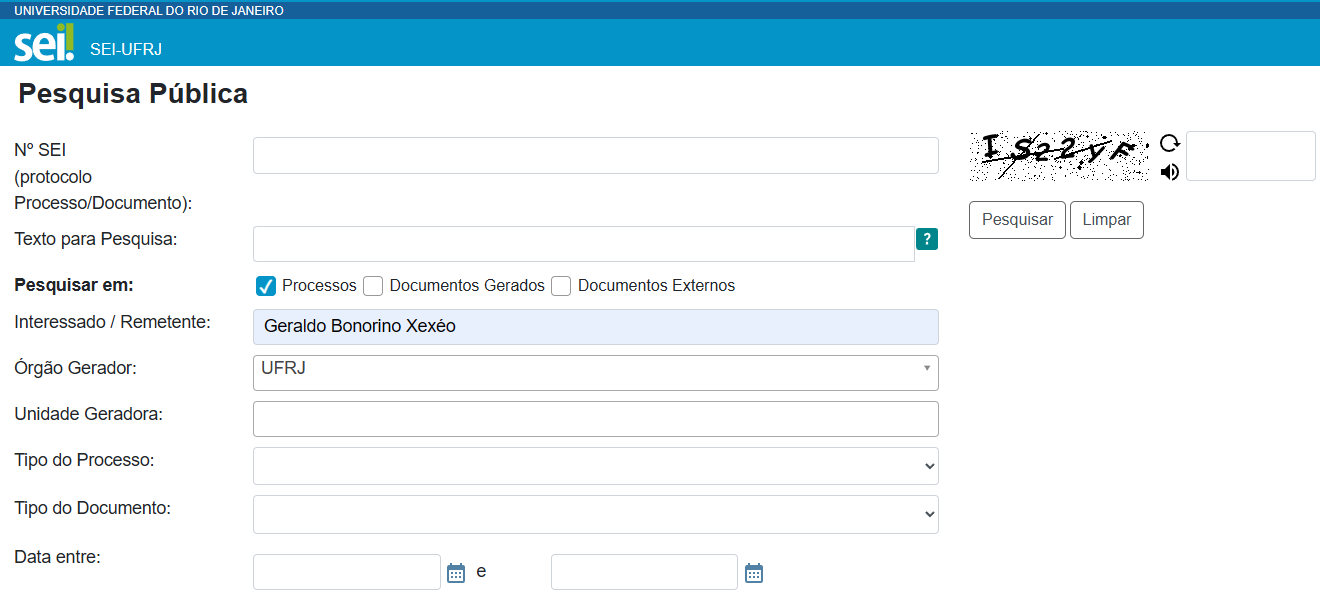
\includegraphics[width=\linewidth]{SEIpesquisa.png}
    \caption{Tela do SEI Pesquisa}
    \label{fig:sei}
\end{figure}

Os processos importantes na defesa são:
\begin{itemize}
    \item Pós-Graduação: Homologação de Candidatura - Qualificação (Stricto Sensu), que tem que estar aprovado para pedir banca.
    \item Pós-Graduação: Aprovação de Banca Examinadora e Homologação de Defesa (Stricto Sensu), que é usado desde o pedido de banca até a entrega do diploma.

\end{itemize}

Outros processos que podem ocorrer:
\begin{itemize}
    \item Pós-Graduação: Mudança de Orientação (Substituição, Inclusão ou Exclusão), se houve mudança na orientação original, como a inclusão de membro externo a Coppe.
    \item Pós-Graduação: Aproveitamento de Disciplina (Stricto Sensu), se foram feitas cadeiras fora da Coppe. 
        \item Pós-Graduação: Prorrogação de Prazo para a Defesa de Dissertação/Tese (Stricto Sensu), se houve prorrogação
\end{itemize}

Os processos são aprovados no PESC, possivelmente pelo Coordenador Acadêmico ou pelo Colegiado em alguns casos, e depois na CPGP. Para saber que um processo foi aprovado é necessário buscar o parecer que indica a aprovação pela CPGP. 

Tirando o período de recesso no fim de ano, a CPGP normalmente se reúne as terças-feiras de manhã e, na quase totalidade dos casos, aprova o parecer do relator, que pode ser favorável, desfavorável, ou fazer exigências. Essas decisões estão listadas como ``Parecer''. Por isso, quando há o parecer favorável do relator, se tem quase certeza que na próxima terça-feira a CPGP aprovará o parecer e o pedido. Se há um parecer desfavorável, ainda há tempo de fazer as correções necessárias.

O professor da COPPE tem acesso a uma interface um pouco mais rica e também experiência em interpretar o que está acontecendo, por exemplo, por que um pedido está parado.



\subsection{Antes da Sua Defesa}

Uma lista de ações obrigatórias para a defesa acontece, e cujas regras variam ao longo do tempo.

\begin{itemize}
    \item Seu orientador deve pedir a banca com até 45 dias de antecedência da data prevista de defesa, que deve ser antes do fim de seu prazo para defesa. 
    \item Você deve depositar a dissertação no registro, provavelmente por meio de uma cópia em PDF salva no software \verb|ctrl-pesc|, \textbf{até 15 dias antes da defesa real (e não da data prevista no pedido)}
    \item Você deve enviar cópias a banca, também até 15 dias antes da defesa, há um documento que informa esse envio ao registro.
    \item A data e o horário finais da defesa tem que ser acordados entre banca e candidato.
    \item Deve ser marcada a sala ou criada a sala virtual.
    \item Deve ser feito um anúncio público e formal da defesa, que será registrado no site do PESC.
    \item O orientador deve pedir a ata para o registro, uns dois ou três dias antes, mas para isso o aluno tem que ter enviado, além da cópia da dissertação em PDF, alguns documentos exigidos pelo registro e que precisam da assinatura do aluno e do orientador. Há um email padrão para isso.
    \item O orientador deve receber a ata digital ou passar no registro para pedir a ata de papel (para isso é necessário avisar antes que vai querer uma ata de papel)
\end{itemize}

\subsubsection{Escolha e convite da banca}

A escolha da banca é uma prerrogativa do orientador. O convite aos membros da banca normalmente é feito pelo orientador. Em alguns casos há uma conversa anterior ao convite oficial para buscar um membro da banca.

Todos os membros da banca devem passar pelo crivo da Coppe, que exige o doutorado e em torno de 1 artigo em revista acadêmica indexada por ano, nos últimos quatro anos, em média. Além disso, é considerada a ligação do membro da banca com o orientador, e a experiência geral do mesmo. Essa análise é feita por meio do currículo Lattes. Isso significa que se um membro proposto não é doutor e não tem pelo menos 3 artigos em revistas indexadas\footnote{Uma revista acadêmica indexada deve constar de índices reconhecidos, principalmente o JCR Web of Science}

\subsubsection{Pedido de banca}

Documento oficial que deve ser feito pelo menos 45 dias antes da defesa. A data marcada no pedido, porém, não é obrigatório. Aprovada a banca, pode ser defendida antes (até agora), ou depois. O procedimento de pedido de banca é iniciado pelo professor, mas depende de documentos do aluno. O pedido é processado pela secretaria acadêmica.

\subsubsection{Reserva de sala}

A sala é reservada na secretaria, com uma pasta específica para isso. Em caso de sala virtual, deve ser divulgado o link e ele deve ser público e aberto para o público. 

\subsection{Depois de Sua Defesa}

Depois de sua defesa a maior parte das obrigações é sua. O orientador apenas vai enviar a ata para o registro. Você deve fazer todo o resto da documentação, no prazo hábil. No caso de reprovação, pouco ou nada há a ser feito.

No caso de aprovação por unanimidade, esse prazo é de 30 dias. Durante esse tempo o orientador deve conversar com você sobre as modificações necessárias a partir dos comentários e perguntas da banca.

No caso de aprovações com exigências, o candidato ainda não foi aprovado. Ao fazer as modificações pedidas o candidato deve prestar contas e interagir com orientador e fiscal.

Nesses dois últimos casos, muito mais frequentes, há vários passos descritos na documentação. Esses passos permitirão que seu diploma seja pedido e seu registro marque que você recebeu o grau de mestre.

Dois passos são importantes, o depósito da versão final da dissertação no registro, para o qual há um prazo fixo e que não pode ser prorrogado, e o depósito da dissertação no PESC, essencial para o prosseguimento do processo de requisição do diploma.

Além disso, é gentil, e praticamente obrigatório, enviar a versão final da dissertação para a banca, em PDF.

\needspace{5\baselineskip}
\section{Comportamento e Preocupações do Candidato}

\subsection{Contagem do Prazo}

O prazo para defesa de dissertação de mestrado e de 3 anos. Ele é contado sempre a partir da data de matrícula no SIGA, que está tanto no Boletim quanto no Histórico Escolar do aluno. Recentemente, a contagem do prazo passou a ser interrompida quando o aluno tranca matrícula, e ainda há outras condições possíveis de interrupção do prazo, como licença médica para maternidade. Esse prazo pode ser prorrogado em até 6 meses, mediante justificativa válida e concordância do orientador.

O pedido de prorrogação, se feito, deve ser feito \textbf{antes do prazo acabar.} O aluno não deve contar com a aprovação\footnote{Não concordarei com pedidos que não sejam embasados em causa grave, o que exclui a falta de tempo por estar trabalhando, e outras condições que poderiam ter sido controladas pelo aluno}.






\subsection{Preparação}

Você deve se preparar para a defesa. No caso de defesa em sala de aula, você deve chegar mais cedo (talvez ir alguns dias antes) para ver como é a sala. 

Deve levar seu próprio computador, um pen-drive de reserva com a apresentação. Não conte com a internet funcionando (Google Slides, por exemplo). Não conte com um computador a sua disposição (apesar de normalmente haver um). 

No caso de defesa remota, você deve ter como fazer a defesa de ``qualquer maneira'', para isso:
\begin{itemize}
    \item Tenha um acesso de internet alternativo. Celulares, por exemplo, podem ser ligados a um computador via USB para funcionarem como modem, ou podem oferecer uma rede wi-fi com a funcionalidade de ``tethering''.
    \item Tenha um computador reserva, pois a casos que o computador dá problema
    \item Verifique antes se câmera, microfone e fone estão funcionando. É essencial que a defesa possua a câmera.
    \item Prepare o celular para backup de câmera, fone e microfone.
    \item Tenha um lugar reserva, pois já aconteceu de ser necessário por falta de luz, internet, etc. 
\end{itemize}

Alguns orientadores fazem uma apresentação prévia\footnote{Não é o meu caso}, outros discutem os slides\footnote{Eu posso rever algumas vezes}. Pergunte o que seu orientador deseja.



\subsection{Slides}

Veja as dicas em \url{https://github.com/xexeo/DicasSlidesAcademicos/blob/main/DicasSlidesAcademicos.pdf}.

Em especial:
\begin{itemize}
    \item Cuidado com ortografia e gramática;
    \item Cuidado com o tamanho de imagens, principalmente nas letras das imagens, para que sejam legíveis;
    \item Numere os slides, e coloque o total de slides;
    \item Não encha os slides de texto;
    \item Não use corpo de fonte menor que 16;
    \item Tente usar corpo 30;
    \item Não faça show de efeitos especiais, mas use se necessário e
    \item Use os logos do Programa, da Coppe e da UFRJ
\end{itemize}

\subsection{Ao apresentar}

Não fique de costas para a banca lendo os slides. Sua apresentação deve ser de frente para a banca e a plateia, sabendo o que vai falar, por isso deve treinar. Não precisa saber de cor. A \autoref{fig:comparacao-apresentacoes} ilustra esse assunto. 

Nem para apontar para o slide fique de costas para a banca, no máximo fique de lado. Olhe para todos na plateia ao longo da apresentação.

Se preciso faça anotações sobre o que deve falar, mas não para ler as anotações, mas de forma que elas possam guiá-lo. Os slides devem funcionar da mesma forma.

\begin{figure}[h!]
    \centering
    \begin{subfigure}[b]{0.45\textwidth}
        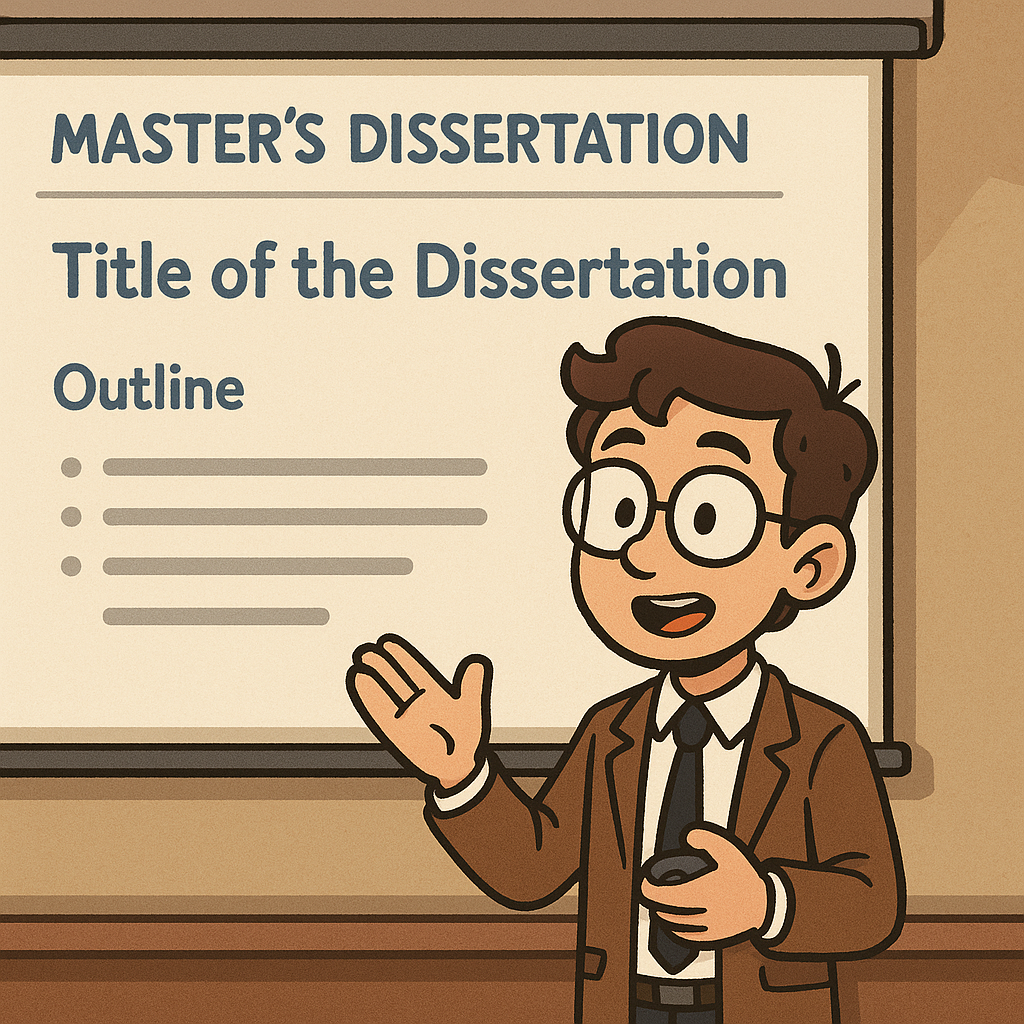
\includegraphics[width=\linewidth]{dando aula.png}
        \caption{Posicionamento correto do candidato.}
        \label{fig:apresentacao-correta}
    \end{subfigure}
    \hfill
    \begin{subfigure}[b]{0.45\textwidth}
        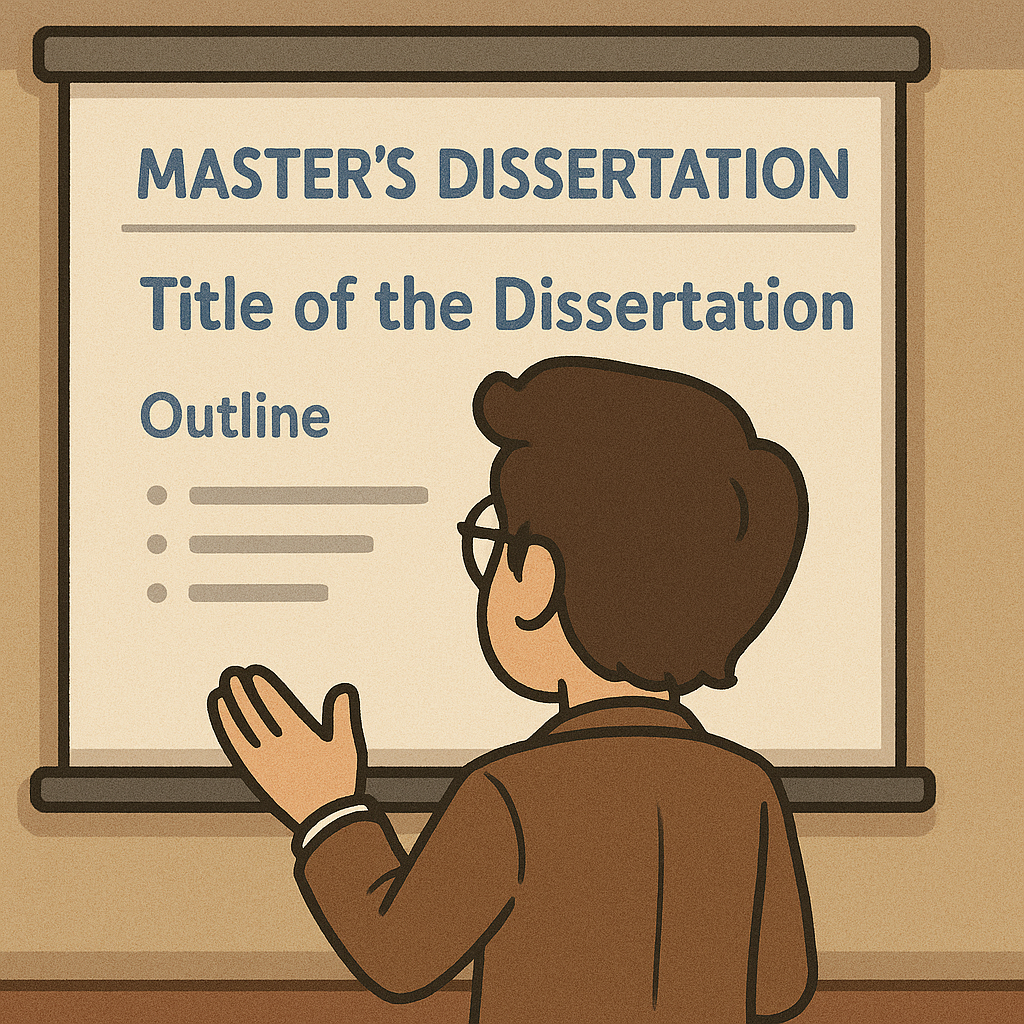
\includegraphics[width=\linewidth]{dando aula errado.png}
        \caption{Posicionamento indevido do candidato.}
        \label{fig:erro-apresentacao}
    \end{subfigure}
    \caption{Comparação entre uma apresentação correta e uma com erro.}
    \label{fig:comparacao-apresentacoes}
\end{figure}



\subsection{Demonstrações de Software}

A melhor forma de demonstrar software é por meio de gravações do sistema funcionando e não rodar diretamente. A experiência prova que é comum que aconteçam problemas de última hora que devem ser evitados. Grave uma utilização e de preferência faça cortes que reduzam os tempos de espera, digitação, etc...

\subsection{Para ficar mais calmo}

É normal ficar nervoso, mas há formas de ajudar a acalmar.
\begin{itemize}
    \item Treine antes, principalmente para fazer a apresentação no tempo. Se você está treinado, vai ficar mais calmo, porque sabe o que tem que fazer.
    \item Tenha com você um copo/garrafa de água, se ficar nervoso, se perder, ou algo assim, pare, respire, tome um gole de água, veja em que ponto está, e então continue com mais calma. O copo de água está ali tanto para matar a sede, como para servir de intervalo sem causar polêmica.
    \item Pelo menos uma vez, no treinamento, grave e veja você apresentando e tente corrigir depois os maus hábitos.
\end{itemize}

\subsection{Durante as perguntas e comentários}

\textbf{Você deve anotar} os que os membros da banca falam. Para isso leve um caderno e caneta. Se quiser gravar (não deixando de anotar), deve pedir autorização. Não anotar é até uma falta de respeito aos comentários da banca. Não é para copiar todas as falas, mas sim deixar um guia para você responder, seja na hora, seja nas correções da dissertação.

Mesmo que o membro da banca fale ``Não precisa anotar porque eu coloquei tudo na dissertação'' ou ``Eu vou te mandar tudo'', anotar é importante para entender o que o membro da banca acha importante, e que perguntas foram feitas.

\subsection{Outras dicas úteis}

Outros documentos que escrevi podem ser úteis, como o \textbf{Dicas para Concurso de Professor}, que discute muito como é feita uma apresentação de uma aula, mas pode ajudar também na defesa da dissertação. Ele pode ser encontrado em:  \url{https://github.com/xexeo/DicasConcursoProvaDeAula/blob/main/discasconcurso.pdf}

\section{Os Resultados}

Existem três resultados possíveis:
\begin{itemize}
    \item \textbf{Aprovação da dissertação por unanimidade}: significa que você foi aprovado sem modificações de relevância. A banca, e a instituição, ainda esperam que algumas modificações sugeridas sejam feitas, e o aluno tem 30 dias para depositar a versão final no registro e no PESC. O orientador pode ou não auxiliar nas modificações, dependendo da importância delas.
    \item \textbf{Aprovação  somente  após  satisfazer  as  exigências que constam 	 na  folha  de   modificações  no  prazo   fixado  pela  banca    ( não superior  a   noventa   dias)}: nesse caso será criada uma ata adicional com uma lista de mudanças, e haverá um ou dois indicados para verificar as modificações foram feitas. Normalmente isso significa que a banca reconhece que foi feito um trabalho que quase atingiu o nível necessário do mestrado, mas que precisa de esforços adicionais, ou que precisa de grandes correções de texto.
    \item \textbf{Reprovação da dissertação}: uma ocorrência rara, mas possível, e provavelmente indicada anteriormente pelo orientador sobre sua possibilidade. Indica que o aluno não atingiu o mínimo desejável para o bter o título de mestrado. Já vi algumas reprovações, sendo que os motivos incluíram plágio, experiências não realizadas, e baixa qualidade total do trabalho que tinha sido avisada pelo orientador.
\end{itemize}



\clearpage
\begin{center}
  \sffamily\Huge\bfseries
  Apêndices
\end{center}

\vspace{1cm} % espaço após o título
\appendix
\section{URLs}

Essas informações foram encontrados quando esse artigo foi escrito, não é possível garantir que estão atualizadas.

\begin{itemize}
\item Site do Programa de Engenharia de Sistemas e Computação (PESC): \url{https://www.cos.ufrj.br/}
    \item Informações sobre o processo de defesa de dissertação de mestrado: \url{https://www.cos.ufrj.br/index.php/pt-BR/academico/302-mestrado-doutorado/6004-defesas-de-dissertacao-de-mestrado-roteiro-completo}
    \item Site da Coppe: \url{https://coppe.ufrj.br/}
    \item Site do Registro Acadêmico da Coppe: \url{https://registro.daac.coppe.ufrj.br/}
    \item Informações sobre depósito pré defesa: \url{https://registro.daac.coppe.ufrj.br/deposito-de-defesas/depositos-2/}
    \item Informações sobre depósito pós defesa: \url{https://registro.daac.coppe.ufrj.br/deposito-de-defesas/deposito-pos-defesa/}
    \item Regimento da Coppe: \url{https://coppe.ufrj.br/regimento-da-coppe-2/}
    \item \textbf{Espaço do Aluno da Coppe}, incluindo a regulamentação e várias decisões importantes referentes a defesas e prazos: \url{https://coppe.ufrj.br/espaco-do-aluno/}
    \item Regulamentação para alunos da Coppe: \url{https://coppe.ufrj.br/wp-content/uploads/2024/06/Alunos_a_partir_2017.1.pdf}
    \item Diretrizes Gerais para Composição de Bancas: \url{http://sokrates.com.br/wp-content/uploads/2025/02/UFRJ_HorizontalCompleta_Tela_Positivo.png}
    \item Acompanhamento de processos no SEI: \url{https://sei.ufrj.br/pesquisa}
\end{itemize}

\clearpage
\section{Checklist de Pré Requisitos}

\begin{itemize}
    \item $\square$ Verificar sua data de matrícula no SIGA e calcular o prazo máximo para defesa.
    \item $\square$ Conferir se já realizou e teve sua candidatura homologada no Seminário de Qualificação do Mestrado.
\end{itemize}
\clearpage
\section{Checklist Pré-Defesa}

\begin{itemize}
    \item $\square$ Discutir a banca com o orientador pelo menos 60 dias antes da defesa.
    \item $\square$ Providenciar o PDF com o currículo Lattes do membro externo da banca, se brasileiro, ou outro currículo, se estrangeiro, e enviar ao orientador.
    \item $\square$ Pedir ao orientador para fazer o pedido de banca com pelo menos 60 dias de antecedência.
    \item $\square$ Garantir que o pedido de banca foi feito com pelo menos 45 dias de antecedência da primeira data planejada.
    \item $\square$ Verificar no SEI a aprovação da banca.
    \item $\square$ Definir a data final da defesa com a banca e orientador.
    \item $\square$ Reservar a sala presencial ou criar o link da sala virtual.
    \item $\square$ Depositar a dissertação (PDF) no \verb|ctrl-pesc| até 15 dias antes da defesa.
    \item $\square$ Enviar o PDF da dissertação a todos os membros da banca até 15 dias antes da defesa.
    \item $\square$ Levantar, preparar, assinar e enviar ao registro e aos orientadores os documentos necessários para pedir a ata, constante da informação de pré-defesa da Coppe.
    \item $\square$ Garantir que o orientador solicitou a ata à secretaria (digital ou física).
    \item $\square$ Confirmar que os documentos obrigatórios foram entregues ao registro (assinados).
    \item $\square$ Confirmar que o orientador divulgou o anúncio formal da defesa no site do PESC (via secretaria).
\end{itemize}
\clearpage
\section{Checklist no Dia da Defesa}

\begin{itemize}
    \item $\square$ Chegar com antecedência à sala física ou testar acesso à sala virtual.
    \item $\square$ Levar computador próprio com a apresentação pronta e funcional offline.
    \item $\square$ Ter pen-drive de backup com os slides.
    \item $\square$ Levar garrafa de água para auxiliar caso haja nervosismo.
    \item $\square$ Conferir funcionamento de câmera, microfone e fones de ouvido.
    \item $\square$ Ter plano B para internet (tethering de celular, etc).
    \item $\square$ Imprimir ou abrir a apresentação com os slides numerados.
    \item $\square$ Conferir se a ata está em posse do presidente da banca.
    \item $\square$ Preparar local alternativo caso haja queda de luz/internet.
    \item $\square$ Conferir que todos os membros da banca estão com o link correto.
    \item $\square$ Ter bloco de anotações (ou editor de texto) para registrar as falas da banca.
\end{itemize}
\clearpage

\section{Checklist Pós-Defesa}

\begin{itemize}
    \item $\square$ Conferir se a ata foi assinada e entregue pelo orientador ao registro.
    \item $\square$ Se aprovado com exigências: seguir instruções da folha de modificações.
    \item $\square$ Entrar em contato com fiscal e orientador para confirmar se as exigências foram cumpridas.
    \item $\square$ Preparar a versão final da dissertação.
    \item $\square$ Depositar a versão final no sistema da Coppe (registro acadêmico), respeitando o prazo.
    \item $\square$ Depositar a versão final no site do PESC.
    \item $\square$ Enviar a versão final (PDF) para todos os membros da banca.
    \item $\square$ Solicitar emissão de diploma após confirmação dos depósitos.
    \item $\square$ Atualizar seu currículo Lattes com o título da dissertação e nome dos orientadores.
\end{itemize}


\end{document}
